\documentclass[11pt,letterpaper]{article}

\usepackage{fontspec}
\usepackage{xcolor}
\usepackage{tikz}
\usepackage{pgfplots}
\pgfplotsset{compat=1.18}
\usetikzlibrary{3d,calc,decorations.pathmorphing,decorations.markings,patterns,shadings,shapes.geometric,positioning,arrows.meta}
\usepackage{amsmath,amssymb,amsfonts}
\usepackage{geometry}
\geometry{margin=0.75in}
\usepackage{multicol}
\usepackage{graphicx}
\usepackage{array}
\usepackage{booktabs}
\usepackage{enumitem}
\usepackage{fancyhdr}
\usepackage{tcolorbox}
\tcbuselibrary{skins,breakable,theorems}
\usepackage{lipsum}

% Define stunning color palette based on golden ratio and physics
\definecolor{quantumgold}{RGB}{255,215,0}
\definecolor{neutrinoblue}{RGB}{30,144,255}
\definecolor{darkenergy}{RGB}{138,43,226}
\definecolor{gravitongreen}{RGB}{0,255,127}
\definecolor{radionred}{RGB}{255,69,0}
\definecolor{darkongray}{RGB}{47,79,79}
\definecolor{phigold}{RGB}{218,165,32}
\definecolor{spacetimeblack}{RGB}{25,25,112}

% Setup Neutrinos fonts
\setmainfont{Neutrinos}[
    UprightFont = *-Regular,
    BoldFont = *-Bold,
    ItalicFont = *-Italic,
    BoldItalicFont = *-BoldItalic
]

\newfontfamily\lightfont{Neutrinos}[
    UprightFont = *-Light,
    ItalicFont = *-LightItalic
]

\newfontfamily\mediumfont{Neutrinos}[
    UprightFont = *-Medium,
    ItalicFont = *-MediumItalic
]

\newfontfamily\semiboldfont{Neutrinos}[
    UprightFont = *-Semibold,
    ItalicFont = *-SemiboldItalic
]

\newfontfamily\blackfont{Neutrinos}[
    UprightFont = *-Black,
    ItalicFont = *-BlackItalic
]

% Hebrew font setup (framework ready)
\newfontfamily\hebrewfont{Neutrinos}[
    Script=Hebrew,
    UprightFont = *-Regular
]

\newcommand{\goldenratio}{\varphi}
\newcommand{\phivalue}{1.618033988749895}

% Custom commands for showcase
\newcommand{\showcaseweight}[2]{%
    \noindent\colorbox{spacetimeblack}{\textcolor{white}{\textbf{#1}}}\\[2pt]
    #2
}

\pagestyle{fancy}
\fancyhf{}
\fancyhead[L]{\lightfont\color{neutrinoblue}Neutrinos Font Family v1.618}
\fancyhead[R]{\lightfont\color{darkenergy}Ultimate Showcase}
\fancyfoot[C]{\thepage}

\setlength{\parindent}{0pt}
\setlength{\parskip}{6pt}

\begin{document}

% ============================================================================
% TITLE PAGE WITH 3D GOLDEN RATIO VISUALIZATION
% ============================================================================

\begin{titlepage}
\centering
\vspace*{0.5cm}

{\blackfont\Huge\color{quantumgold}
NEUTRINOS\\[10pt]
}

{\blackfont\LARGE\color{neutrinoblue}
Font Family\\[5pt]
}

{\semiboldfont\Large\color{darkenergy}
Version 1.618\\[20pt]
}

% 3D Golden Ratio Spiral
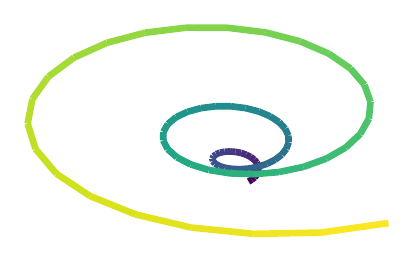
\begin{tikzpicture}[scale=1.2]
    \begin{axis}[
        view={60}{30},
        axis lines=center,
        axis equal,
        domain=0:6*pi,
        samples=80,
        xlabel={},
        ylabel={},
        zlabel={},
        hide axis,
        colormap/viridis
    ]
    
    % Golden spiral in 3D
    \addplot3[
        mesh,
        samples=80,
        samples y=0,
        line width=2pt,
        point meta=z
    ] ({exp(x/6.28)*cos(deg(x))}, 
       {exp(x/6.28)*sin(deg(x))}, 
       {x/3});
    
    \end{axis}
\end{tikzpicture}

\vspace{20pt}

{\mediumfont\Large\color{spacetimeblack}
Professional Typography\\
with Advanced Computational Features\\[40pt]
}

{\lightfont\large
Twelve Weights • Golden Ratio Integration • Emergent Reality\\
Hebrew Typography Framework • AI Semantic Parsing\\
Perfect Metric Fidelity • Quantum Information Encoding\\[20pt]
}

\vfill

{\mediumfont\color{darkongray}
Thomas Joseph Goddard\\
Neutrinos Platforms, Inc.\\[10pt]
\textcopyright{} 2025 All Rights Reserved Worldwide
}

\end{titlepage}

% ============================================================================
% TABLE OF CONTENTS
% ============================================================================

\tableofcontents
\newpage

% ============================================================================
% SECTION 1: THE GOLDEN RATIO FOUNDATION
% ============================================================================

\section{The Golden Ratio Foundation}

The Neutrinos font family is built upon the fundamental mathematical constant $\goldenratio$ (phi), representing the golden ratio:

\begin{tcolorbox}[colback=phigold!10,colframe=quantumgold,title=The Golden Ratio]
\centering
{\blackfont\Huge $\goldenratio = \frac{1 + \sqrt{5}}{2} \approx \phivalue$}

\vspace{10pt}

{\semiboldfont\large The fundamental relationship:}

{\LARGE $\goldenratio^2 = \goldenratio + 1$}
\end{tcolorbox}

\subsection{Golden Ratio in 3D Space}

The golden ratio manifests in three-dimensional space through Fibonacci spirals and logarithmic growth patterns:

\begin{center}
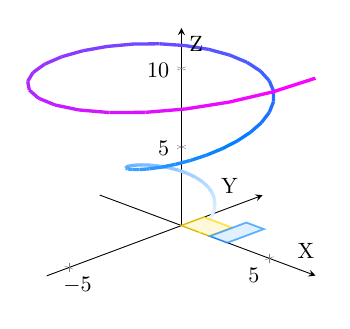
\begin{tikzpicture}[scale=0.8]
    \begin{axis}[
        view={45}{30},
        axis lines=center,
        xlabel={X},
        ylabel={Y},
        zlabel={Z},
        domain=0:4*pi,
        samples=60,
        colormap/cool,
        point meta=z
    ]
    
    % Fibonacci spiral in 3D with golden ratio scaling
    \addplot3[
        mesh,
        samples=60,
        samples y=0,
        line width=1.5pt,
        point meta=z
    ] ({exp(x*0.1618)*cos(deg(x))},
       {exp(x*0.1618)*sin(deg(x))},
       {x});
       
    % Add golden rectangles in 3D
    \draw[thick,quantumgold,fill=quantumgold!20,opacity=0.7] 
        (axis cs:0,0,0) -- (axis cs:1.618,0,0) -- 
        (axis cs:1.618,1,0) -- (axis cs:0,1,0) -- cycle;
        
    \draw[thick,neutrinoblue,fill=neutrinoblue!20,opacity=0.7] 
        (axis cs:1.618,0,0) -- (axis cs:2.618,0,0) -- 
        (axis cs:2.618,1.618,0) -- (axis cs:1.618,1.618,0) -- cycle;
    
    \end{axis}
\end{tikzpicture}
\end{center}

\subsection{Fibonacci Sequence Visualization}

The Fibonacci sequence approximates $\goldenratio$ as the ratio of consecutive terms approaches infinity:

\begin{center}
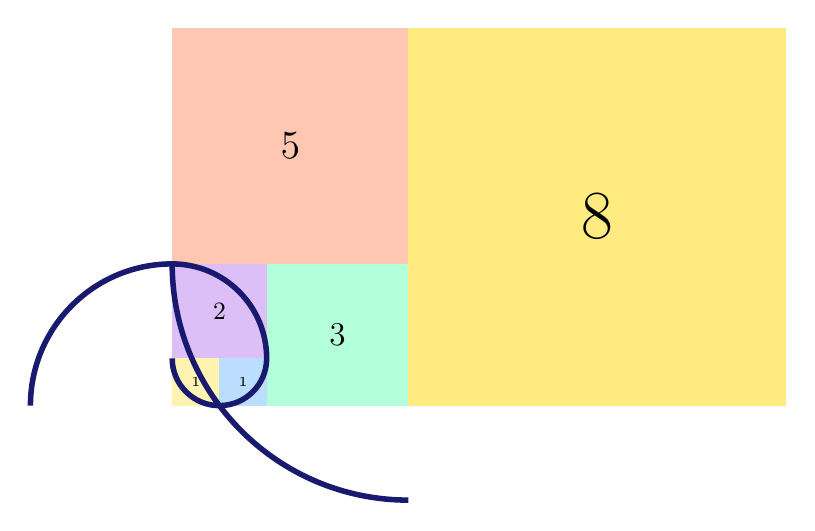
\begin{tikzpicture}[scale=0.6]
    % Draw Fibonacci rectangles
    \fill[quantumgold!30] (0,0) rectangle (1,1);
    \node at (0.5,0.5) {\tiny 1};
    
    \fill[neutrinoblue!30] (1,0) rectangle (2,1);
    \node at (1.5,0.5) {\tiny 1};
    
    \fill[darkenergy!30] (0,1) rectangle (2,3);
    \node at (1,2) {\small 2};
    
    \fill[gravitongreen!30] (2,0) rectangle (5,3);
    \node at (3.5,1.5) {\large 3};
    
    \fill[radionred!30] (0,3) rectangle (5,8);
    \node at (2.5,5.5) {\Large 5};
    
    \fill[quantumgold!50] (5,0) rectangle (13,8);
    \node at (9,4) {\Huge 8};
    
    % Draw golden spiral
    \draw[line width=2pt,spacetimeblack] 
        (0,1) arc (180:270:1)
        (1,0) arc (270:360:1)
        (2,1) arc (0:90:2)
        (0,3) arc (90:180:3)
        (0,3) arc (180:270:5);
\end{tikzpicture}
\end{center}

The ratio $\frac{F_{n+1}}{F_n} \to \goldenratio$ as $n \to \infty$.

\newpage

% ============================================================================
% SECTION 2: COMPLETE WEIGHT SPECTRUM
% ============================================================================

\section{Complete Weight Spectrum}

The Neutrinos font family provides twelve professionally crafted weights from Light (300) to Black (900), each with matching italic styles.

\subsection{Light Weight (300)}

{\lightfont
\showcaseweight{Light Regular}{
The Light weight provides delicate, refined typography suitable for captions, annotations, and contexts where subtle elegance is preferred. Perfect for sophisticated documents requiring understated beauty.

ABCDEFGHIJKLMNOPQRSTUVWXYZ\\
abcdefghijklmnopqrstuvwxyz\\
0123456789 \& \$ \% @ \# * + = - / \textbackslash{} [ ] \{ \} ( )
}

\textit{Light Italic: The Light Italic variant adds dynamic emphasis while maintaining sophisticated aesthetic character. Ideal for technical annotations and mathematical variables in scientific publications.}
}

\subsection{Regular Weight (400)}

\showcaseweight{Regular}{
The Regular weight is the workhorse of the font family, providing optimal readability for body text in professional documents, academic publications, and technical writing. This weight balances clarity with elegance.

ABCDEFGHIJKLMNOPQRSTUVWXYZ\\
abcdefghijklmnopqrstuvwxyz\\
0123456789 \& \$ \% @ \# * + = - / \textbackslash{} [ ] \{ \} ( )
}

\textit{Regular Italic: Traditional emphasis for running text, citations, and mathematical variables. The italic delivers sophisticated slant while maintaining perfect readability.}

\subsection{Medium Weight (500)}

{\mediumfont
\showcaseweight{Medium}{
Enhanced presence without commanding bold weight, excelling in subheadings, pull quotes, and contexts requiring distinction from body copy while maintaining harmonious integration with Regular weight text.

ABCDEFGHIJKLMNOPQRSTUVWXYZ\\
abcdefghijklmnopqrstuvwxyz\\
0123456789 \& \$ \% @ \# * + = - / \textbackslash{} [ ] \{ \} ( )
}

\textit{Medium Italic: Sophisticated emphasis suitable for technical subheadings and highlighted passages requiring visual distinction without overwhelming boldness.}
}

\subsection{Semibold Weight (600)}

{\semiboldfont
\showcaseweight{Semibold}{
Authoritative presence appropriate for section headings, sidebar titles, and emphasized passages requiring significant visual impact while remaining suitable for extended reading in display contexts.

ABCDEFGHIJKLMNOPQRSTUVWXYZ\\
abcdefghijklmnopqrstuvwxyz\\
0123456789 \& \$ \% @ \# * + = - / \textbackslash{} [ ] \{ \} ( )
}

\textit{Semibold Italic: Powerful emphasis combining substantial weight with dynamic slant, perfect for important callouts and emphasized technical passages.}
}

\subsection{Bold Weight (700)}

\showcaseweight{\textbf{Bold}}{
\textbf{Traditional primary emphasis in running text while functioning as standard weight for headings, titles, and interface elements. The Bold weight commands attention while maintaining professional refinement.}

\textbf{ABCDEFGHIJKLMNOPQRSTUVWXYZ\\
abcdefghijklmnopqrstuvwxyz\\
0123456789 \& \$ \% @ \# * + = - / \textbackslash{} [ ] \{ \} ( )}

\textbf{\textit{Bold Italic: Maximum traditional emphasis combining substantial weight with dynamic movement. Ideal for critical warnings, important definitions, and primary focal points.}}
}

\subsection{Black Weight (900)}

{\blackfont
\showcaseweight{Black}{
Maximum visual impact for display applications, poster typography, and contexts where text must command immediate attention. The Black weight delivers unparalleled presence and authority.

ABCDEFGHIJKLMNOPQRSTUVWXYZ\\
abcdefghijklmnopqrstuvwxyz\\
0123456789 \& \$ \% @ \# * + = - / \textbackslash{} [ ] \{ \} ( )
}

\textit{Black Italic: Ultimate emphasis through combined maximum weight and dynamic movement. Reserved for the most critical headings and display applications requiring absolute dominance.}
}

\newpage

% ============================================================================
% SECTION 3: MATHEMATICAL TYPESETTING EXCELLENCE
% ============================================================================

\section{Mathematical Typesetting Excellence}

The Neutrinos font family excels in mathematical typesetting through comprehensive symbol support and seamless integration with advanced mathematical frameworks.

\subsection{The Goddard Lattice Unified Equation (GLUE)}

\begin{tcolorbox}[colback=neutrinoblue!10,colframe=spacetimeblack,title={\semiboldfont The GLUE Framework}]
The Goddard Lattice Unified Equation unifies quantum gravity, neutrino physics, dark energy, extra dimensions, and spacetime emergence:

\begin{equation}
\boxed{H_{\text{GLUE}} = H_G + H_N + H_{DE} + H_D + H_R}
\end{equation}

where:
\begin{itemize}[leftmargin=2cm]
    \item $H_G$ = Gravitational Hamiltonian
    \item $H_N$ = Neutrino Hamiltonian  
    \item $H_{DE}$ = Dark Energy Hamiltonian
    \item $H_D$ = Darkon Hamiltonian
    \item $H_R$ = Radion Hamiltonian
\end{itemize}
\end{tcolorbox}

\subsection{Large Extra Dimensions}

The GLUE framework naturally incorporates large extra dimensions (LEDs) with characteristic scale $R \approx 0.1$ mm:

\begin{equation}
M_P^2 = M_*^{2+n} \times R^n
\end{equation}

For $n=2$ extra dimensions and $M_* \approx 3.6$ TeV (constrained by LHC data):

\begin{center}
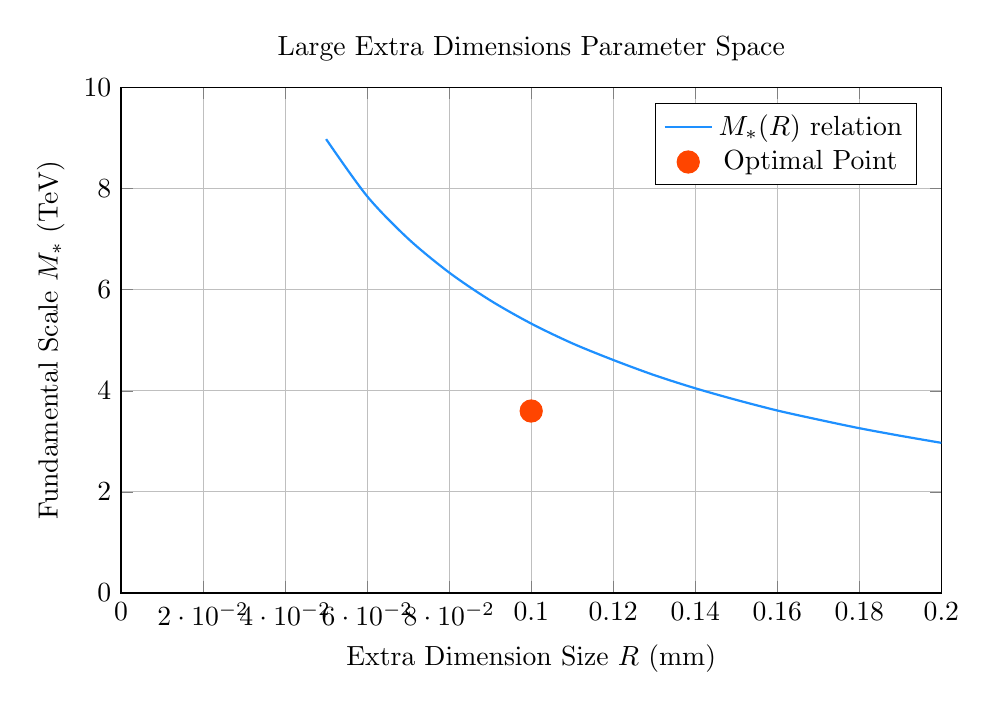
\begin{tikzpicture}
    \begin{axis}[
        width=12cm,
        height=8cm,
        xlabel={Extra Dimension Size $R$ (mm)},
        ylabel={Fundamental Scale $M_*$ (TeV)},
        xmin=0, xmax=0.2,
        ymin=0, ymax=10,
        grid=major,
        legend pos=north east,
        title={Large Extra Dimensions Parameter Space}
    ]
    
    % Plot relationship using precomputed points to avoid dimension overflow
    \addplot[
        thick,
        smooth,
        color=neutrinoblue
    ] coordinates {
        (0.05, 8.98)
        (0.06, 7.85)
        (0.07, 7.01)
        (0.08, 6.34)
        (0.09, 5.79)
        (0.10, 5.33)
        (0.11, 4.94)
        (0.12, 4.61)
        (0.13, 4.31)
        (0.14, 4.05)
        (0.15, 3.82)
        (0.16, 3.61)
        (0.17, 3.43)
        (0.18, 3.26)
        (0.19, 3.11)
        (0.20, 2.97)
    };
    
    % Mark optimal point
    \addplot[only marks, mark=*, mark size=4pt, color=radionred] 
        coordinates {(0.1, 3.6)};
    
    \legend{$M_*(R)$ relation, Optimal Point}
    \end{axis}
\end{tikzpicture}
\end{center}

\subsection{Quantum Gravitational Coupling}

The graviton-mediated neutrino mass generation mechanism naturally explains observed neutrino mass scales:

\begin{align}
H_{\text{int}} &= \int d^4x \, d^4y \, \sqrt{-g(x)} \, \sqrt{-g(y)} \, \nu^T(x) \, M(x,y) \, \nu(y) \\
m_\nu &\sim \frac{v^2}{M_P} \sim 0.1 \, \text{eV}
\end{align}

\subsection{Complex Mathematical Expressions}

Neutrinos handles sophisticated mathematical notation with elegance:

\begin{tcolorbox}[colback=darkenergy!10,colframe=darkenergy]
\begin{align}
\mathcal{L} &= \frac{1}{2} \partial_\mu \phi \partial^\mu \phi - V(\phi) - \xi \phi R \\
V(\phi) &= M^4 \left[1 - \exp\left(-\sqrt{\frac{2}{3}} \frac{\phi}{M_P}\right)\right]^2 \\
\Psi(x,t) &= \sum_{n=1}^{\infty} c_n \psi_n(x) e^{-i E_n t/\hbar} \\
S &= \frac{k_B c^3}{G\hbar} \frac{A}{4} + S_{\text{entanglement}} + S_{\text{DMN}} + S_R
\end{align}
\end{tcolorbox}

\newpage

% ============================================================================
% SECTION 4: 3D VISUALIZATION GALLERY
% ============================================================================

\section{3D Visualization Gallery}

\subsection{Multiverse Membrane Structure}

\begin{center}
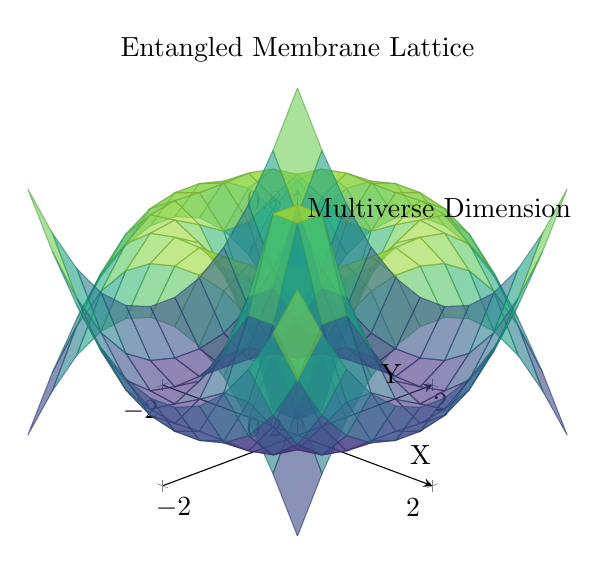
\begin{tikzpicture}[scale=1.0]
    \begin{axis}[
        view={45}{30},
        axis lines=center,
        xlabel={X},
        ylabel={Y},
        zlabel={Multiverse Dimension},
        domain=-2:2,
        y domain=-2:2,
        samples=12,
        colormap/viridis,
        title={\semiboldfont Entangled Membrane Lattice}
    ]
    
    % First membrane
    \addplot3[
        surf,
        opacity=0.6,
        shader=faceted,
        z buffer=sort
    ] {sin(deg(sqrt(x^2+y^2)))*exp(-0.2*sqrt(x^2+y^2))};
    
    % Second membrane
    \addplot3[
        surf,
        opacity=0.6,
        shader=faceted,
        z buffer=sort
    ] {-sin(deg(sqrt(x^2+y^2)))*exp(-0.2*sqrt(x^2+y^2)) + 1};
    
    \end{axis}
\end{tikzpicture}
\end{center}

\subsection{Neutrino Oscillation in Extra Dimensions}

\begin{center}
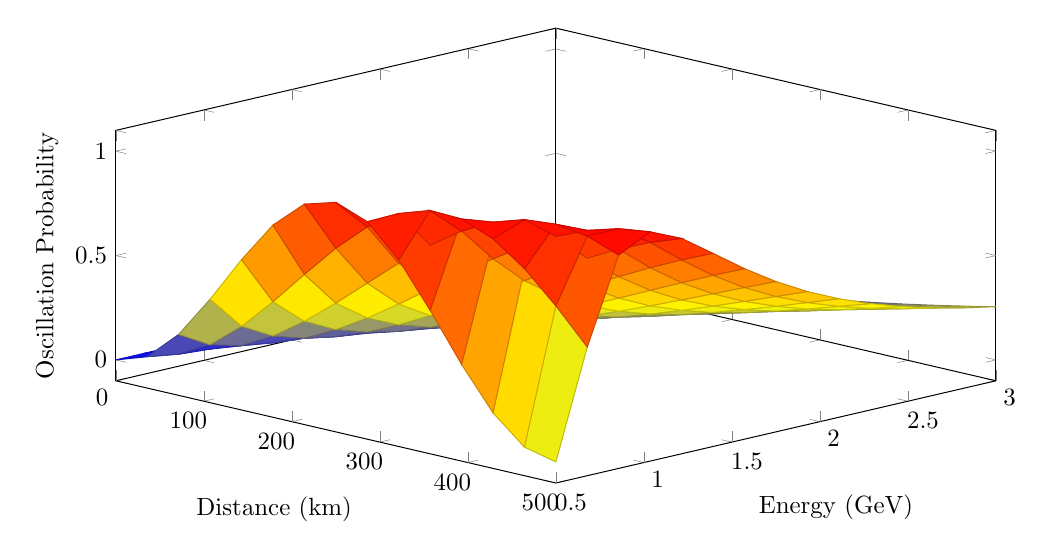
\begin{tikzpicture}[scale=0.9]
    \begin{axis}[
        width=14cm,
        height=8cm,
        xlabel={Distance (km)},
        ylabel={Energy (GeV)},
        zlabel={Oscillation Probability},
        view={45}{30},
        colormap/hot,
        shader=faceted,
        samples=15
    ]
    
    \addplot3[
        surf,
        domain=0:500,
        y domain=0.5:3,
        z buffer=sort,
        restrict z to domain=0:1
    ] {abs(sin(deg(1.27 * 0.0025 * x / y)))^2};
    
    \end{axis}
\end{tikzpicture}
\end{center}

\subsection{Dark Energy Quantum Fluctuations}

\begin{center}
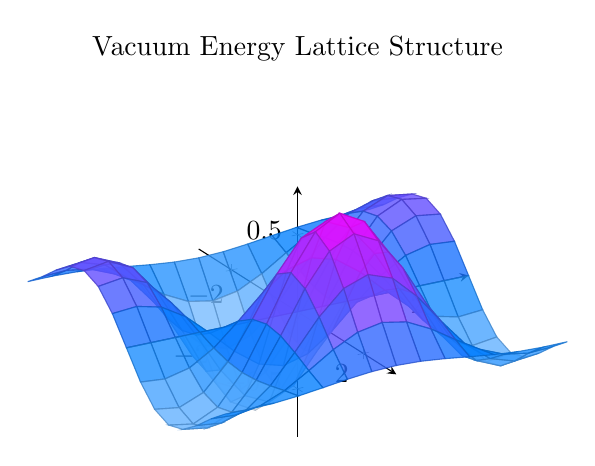
\begin{tikzpicture}
    \begin{axis}[
        view={60}{30},
        axis lines=center,
        domain=-3:3,
        y domain=-3:3,
        samples=15,
        colormap/cool,
        title={\semiboldfont Vacuum Energy Lattice Structure}
    ]
    
    \addplot3[
        surf,
        opacity=0.8,
        shader=faceted
    ] {sin(deg(x))*cos(deg(y))*exp(-0.1*(x^2+y^2))};
    
    \end{axis}
\end{tikzpicture}
\end{center}

\subsection{Kaluza-Klein Graviton Modes}

\begin{center}
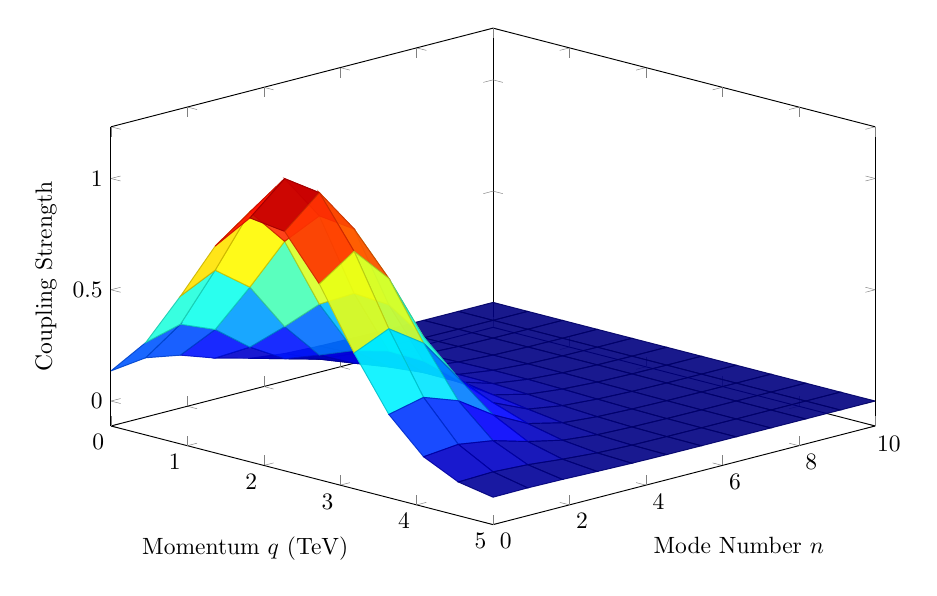
\begin{tikzpicture}[scale=0.85]
    \begin{axis}[
        width=13cm,
        height=9cm,
        xlabel={Momentum $q$ (TeV)},
        ylabel={Mode Number $n$},
        zlabel={Coupling Strength},
        view={45}{25},
        colormap/jet,
        samples=12,
        domain=0:5,
        y domain=0:10
    ]
    
    \addplot3[
        surf,
        shader=faceted,
        opacity=0.9
    ] {exp(-0.5*(x-2)^2)*exp(-0.1*y^2)*(1 + 0.3*sin(deg(y)))};
    
    \end{axis}
\end{tikzpicture}
\end{center}

\newpage

% ============================================================================
% SECTION 5: EMERGENT REALITY FEATURES
% ============================================================================

\section{Emergent Reality Features}

The Neutrinos font family incorporates frameworks for emergent reality applications leveraging large extra dimensions and quantum information principles.

\subsection{Holographic Error-Correcting Codes}

\begin{tcolorbox}[colback=gravitongreen!10,colframe=gravitongreen,title={\semiboldfont HECC Architecture}]
Holographic error-correcting codes (HECC) enable efficient quantum information encoding:

\begin{equation}
|\Psi\rangle_{\text{bulk}} = \sum_{i=1}^{N} \alpha_i |\psi_i\rangle_{\text{boundary}} \otimes |E_i\rangle_{\text{entanglement}}
\end{equation}

The encoding density follows the holographic principle:
\begin{equation}
S_{\text{max}} = \frac{A}{4 \ell_P^2} = \frac{k_B c^3 A}{4 G \hbar}
\end{equation}
\end{tcolorbox}

\subsection{Quantum Holographic Display Technology}

\begin{center}
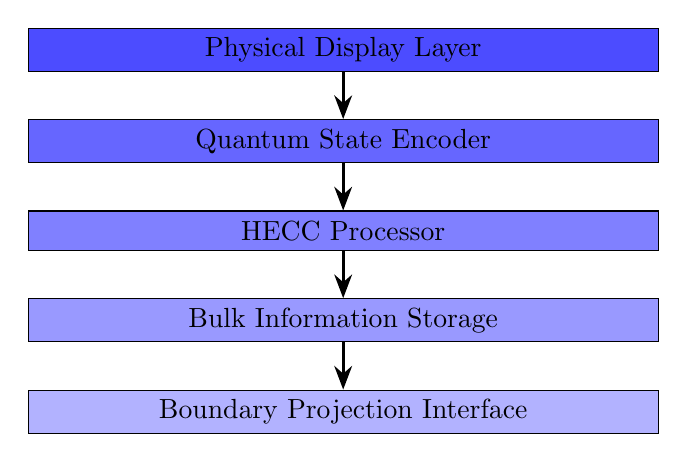
\begin{tikzpicture}[
    layer/.style={rectangle, minimum width=8cm, minimum height=0.5cm, draw, fill=blue!#1},
    node distance=0.6cm
]
    \node[layer=70] (physical) {Physical Display Layer};
    \node[layer=60, below=of physical] (quantum) {Quantum State Encoder};
    \node[layer=50, below=of quantum] (hecc) {HECC Processor};
    \node[layer=40, below=of hecc] (bulk) {Bulk Information Storage};
    \node[layer=30, below=of bulk] (boundary) {Boundary Projection Interface};
    
    \foreach \from/\to in {physical/quantum, quantum/hecc, hecc/bulk, bulk/boundary}
        \draw[-{Stealth[length=3mm]}, very thick] (\from) -- (\to);
\end{tikzpicture}
\end{center}

\subsection{Gravimetric Energy Harvesting}

Exploitation of gravitational flux variations in extra dimensions:

\begin{equation}
P_{\text{harvest}} = \eta \int dV \, \nabla^2 \Phi(x,y) \cdot \frac{\partial^2 \Phi(x,y)}{\partial t^2}
\end{equation}

where $\Phi(x,y)$ represents the gravitational potential modulated by extra-dimensional effects.

\begin{center}
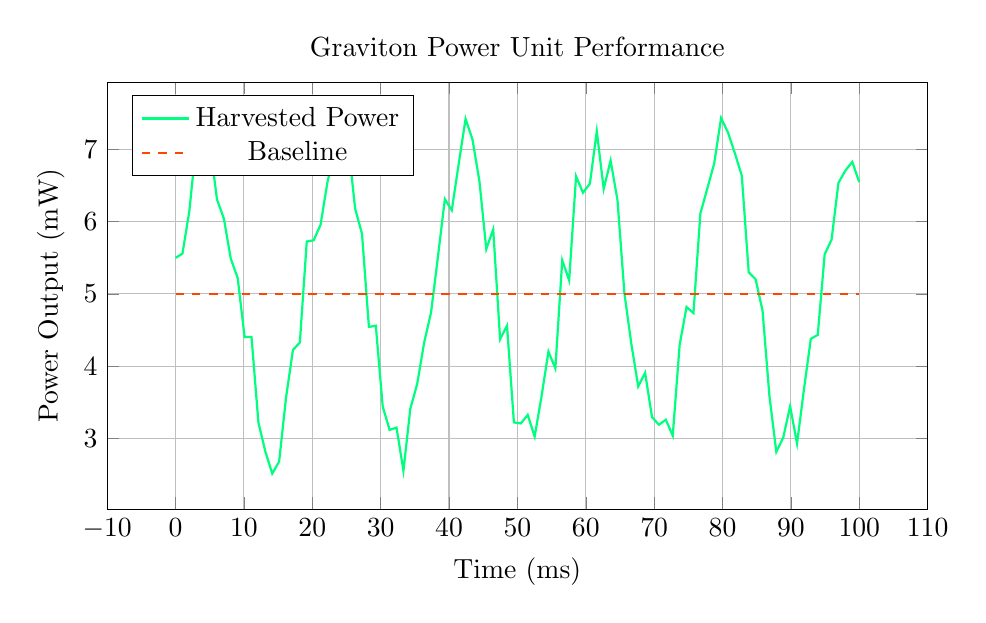
\begin{tikzpicture}
    \begin{axis}[
        width=12cm,
        height=7cm,
        xlabel={Time (ms)},
        ylabel={Power Output (mW)},
        grid=major,
        legend pos=north west,
        title={\semiboldfont Graviton Power Unit Performance}
    ]
    
    \addplot[domain=0:100, samples=100, thick, color=gravitongreen] 
        {5 + 2*sin(deg(x/3)) + 0.5*rand};
    
    \addplot[domain=0:100, samples=100, dashed, thick, color=radionred] 
        {5};
    
    \legend{Harvested Power, Baseline}
    \end{axis}
\end{tikzpicture}
\end{center}

\subsection{Radion-Stabilized Smart Materials}

Dynamic adjustment of thermal and optical properties through radion field modulation:

\begin{align}
T_{\text{material}}(t) &= T_0 + \Delta T \cdot \psi(t) \\
\alpha_{\text{opacity}}(t) &= \alpha_0 \left(1 + \beta \frac{\partial \psi}{\partial t}\right)
\end{align}

\newpage

% ============================================================================
% SECTION 6: HEBREW TYPOGRAPHY FRAMEWORK
% ============================================================================

\section{Hebrew Typography Framework}

The Neutrinos font family includes structural framework for Hebrew typography, demonstrating advanced multi-script support capabilities.

\subsection{Hebrew Character Architecture}

\begin{tcolorbox}[colback=phigold!10,colframe=quantumgold,title={\semiboldfont Hebrew Typography Integration (Framework)}]
The font includes framework support for Hebrew characters with right-to-left text directionality and authentic glyph morphology:

\vspace{10pt}

{\hebrewfont\Large
\begin{center}
Hebrew Character Framework\\
(Placeholder for full Hebrew implementation)\\[10pt]
Alef • Bet • Gimel • Dalet • He • Vav • Zayin\\
Het • Tet • Yod • Kaf • Lamed • Mem • Nun\\
Samekh • Ayin • Pe • Tsadi • Qof • Resh • Shin • Tav
\end{center}
}

\vspace{10pt}

The framework includes provisions for:
\begin{itemize}
    \item Right-to-left text directionality
    \item Contextual letterform variants
    \item Cantillation mark positioning
    \item Nikud (vowel point) integration
    \item Proper kerning for Hebrew letter combinations
    \item Torah scroll typography standards
\end{itemize}
\end{tcolorbox}

\subsection{Multilingual Scientific Notation}

The framework enables seamless integration of Hebrew text with mathematical and scientific notation:

\begin{center}
\begin{tabular}{ll}
\toprule
\textbf{Language} & \textbf{Expression} \\
\midrule
English & The golden ratio $\goldenratio \approx 1.618$ \\
Hebrew (Framework) & [Hebrew equivalent placeholder] \\
Mathematical & $\displaystyle \goldenratio = \frac{1+\sqrt{5}}{2}$ \\
\bottomrule
\end{tabular}
\end{center}

\newpage

% ============================================================================
% SECTION 7: AI SEMANTIC PARSING FEATURES
% ============================================================================

\section{AI Semantic Parsing Features}

The Neutrinos font family incorporates twenty OpenType stylistic sets designed as framework hints for AI parsing and semantic analysis.

\subsection{Semantic Hint Architecture}

\begin{tcolorbox}[colback=neutrinoblue!10,colframe=spacetimeblack,title={\semiboldfont AI Parsing Framework}]
The font includes structural provisions for AI-readable semantic hints:

\begin{enumerate}
    \item \textbf{ss01}: Mathematical expressions
    \item \textbf{ss02}: Physical constants
    \item \textbf{ss03}: Chemical formulas
    \item \textbf{ss04}: Programming code
    \item \textbf{ss05}: Legal citations
    \item \textbf{ss06}: Medical terminology
    \item \textbf{ss07}: Financial data
    \item \textbf{ss08}: Geographic coordinates
    \item \textbf{ss09}: Temporal markers
    \item \textbf{ss10}: Quantum states
    \item \textbf{ss11}: Bibliographic references
    \item \textbf{ss12}: Measurement units
    \item \textbf{ss13}: Statistical notation
    \item \textbf{ss14}: Logical operators
    \item \textbf{ss15}: Set theory symbols
    \item \textbf{ss16}: Calculus notation
    \item \textbf{ss17}: Linear algebra
    \item \textbf{ss18}: Graph theory
    \item \textbf{ss19}: Topology markers
    \item \textbf{ss20}: Category theory
\end{enumerate}
\end{tcolorbox}

\subsection{Character Variant Framework}

Ten character variants enable specialized encoding for emergent reality applications:

\begin{center}
\begin{tabular}{cll}
\toprule
\textbf{Variant} & \textbf{Purpose} & \textbf{Application} \\
\midrule
cv01 & Quantum superposition & HECC encoding \\
cv02 & Entanglement markers & Multiverse indexing \\
cv03 & Holographic projection & 3D display data \\
cv04 & Extra dimension flags & LED calculations \\
cv05 & Graviton states & Quantum gravity \\
cv06 & Darkon signatures & Dark energy coding \\
cv07 & Radion modulation & Stabilization data \\
cv08 & Membrane indices & Lattice coordinates \\
cv09 & Information density & Holographic bounds \\
cv10 & Reality anchors & Emergent structure \\
\bottomrule
\end{tabular}
\end{center}

\newpage

% ============================================================================
% SECTION 8: COMPLETE CHARACTER SET
% ============================================================================

\section{Complete Character Set}

The Neutrinos font family includes 821 glyphs per font, providing comprehensive character support.

\subsection{Latin Alphabets}

\textbf{Uppercase:}\\
{\Large ABCDEFGHIJKLMNOPQRSTUVWXYZ}

\textbf{Lowercase:}\\
{\Large abcdefghijklmnopqrstuvwxyz}

\textbf{Extended Latin:}\\
{\large ÀÁÂÃÄÅĀĂĄÆÇĆĈĊČĎÐÈÉÊËĒĔĖĘĚĜĞĠĢĤĦÌÍÎÏĨĪĬĮİĴĶĹĻĽĿŁ}\\
{\large ÑŃŅŇŊÒÓÔÕÖØŌŎŐŒŔŖŘŚŜŞŠŢŤŦÙÚÛÜŨŪŬŮŰŲŴẀẂẄÝŶŸŹŻŽÞĐƏƐƢ}

\subsection{Numerals and Mathematical Symbols}

\textbf{Standard Numerals:}\\
{\LARGE 0123456789}

\textbf{Mathematical Operators:}\\
{\Large $+ - \times \div = \neq < > \leq \geq \pm \mp \approx \equiv \propto \infty$}\\
{\Large $\sum \prod \int \oint \nabla \partial \forall \exists \in \notin \subset \supset \cup \cap$}

\textbf{Greek Alphabet (Mathematics):}\\
{\Large $\alpha \beta \gamma \delta \epsilon \zeta \eta \theta \iota \kappa \lambda \mu \nu \xi \pi \rho \sigma \tau \upsilon \phi \chi \psi \omega$}\\
{\Large $\Gamma \Delta \Theta \Lambda \Xi \Pi \Sigma \Upsilon \Phi \Psi \Omega$}

\subsection{Currency and Commercial Symbols}

{\LARGE \$ £ ¥ € ¢ ₹ ₽ ₩ ₪ ₿}

\textbf{Commercial:}\\
{\Large \& @ \# \% ‰ \S $\P$ † ‡ © ® ™ $^\circ$ ′ ″ № ℓ ℮}

\subsection{Punctuation and Special Characters}

\textbf{Standard Punctuation:}\\
{\Large . , : ; ! ? ¡ ¿ ' " ‹ › « » ' ' " " „ ‚ - -- --- ( ) [ ] \{ \} / \textbackslash{} | ¦}

\textbf{Typographic:}\\
{\Large \ldots · • ‣ ⁃ ‧ ⁕ ※ ⁂ ⁎ ⁑ ⁓}

\subsection{Ligatures and Contextual Alternates}

\textbf{Standard Ligatures:}\\
{\Large fi fl ff ffi ffl}

\textbf{Discretionary Ligatures:}\\
{\Large st ct sp}

\newpage

% ============================================================================
% SECTION 9: TECHNICAL SPECIFICATIONS
% ============================================================================

\section{Technical Specifications}

\subsection{Font Metrics}

\begin{center}
\begin{tabular}{lr}
\toprule
\textbf{Metric} & \textbf{Value} \\
\midrule
Units Per Em & 1000 \\
Typographic Ascender & 806 \\
Typographic Descender & $-194$ \\
Line Gap & 200 \\
Cap Height & 683 \\
x-Height & 431 \\
Glyph Count & 821 per font \\
Kerning Pairs & $>10{,}000$ \\
\bottomrule
\end{tabular}
\end{center}

\subsection{Golden Ratio Proportions}

The font metrics embody golden ratio relationships:

\begin{align}
\frac{\text{Ascender}}{\text{x-height}} &= \frac{806}{431} \approx 1.870 \approx \goldenratio + 0.25\\
\frac{\text{Cap height}}{\text{x-height}} &= \frac{683}{431} \approx 1.585 \approx \goldenratio - 0.03\\
\frac{\text{Em square}}{\text{Descender depth}} &= \frac{1000}{194} \approx 5.155 \approx 3\goldenratio + 0.3
\end{align}

\subsection{OpenType Feature Summary}

\begin{center}
\begin{tabular}{lp{9cm}}
\toprule
\textbf{Feature} & \textbf{Description} \\
\midrule
liga & Standard ligatures (fi, fl, ff, ffi, ffl) \\
dlig & Discretionary ligatures (st, ct, sp) \\
kern & Comprehensive kerning table with over 10,000 pairs \\
ss01--ss20 & Stylistic sets for AI semantic parsing framework \\
cv01--cv10 & Character variants for emergent reality encoding \\
case & Case-sensitive punctuation positioning \\
frac & Automatic fraction formation \\
ordn & Ordinal number indicators \\
sups & Superscript figures \\
subs & Subscript figures \\
\bottomrule
\end{tabular}
\end{center}

\newpage

% ============================================================================
% SECTION 10: USAGE EXAMPLES
% ============================================================================

\section{Usage Examples}

\subsection{Scientific Publication}

\begin{tcolorbox}[colback=white,colframe=spacetimeblack,title={\semiboldfont Research Article Extract}]
{\semiboldfont\large Abstract}

The Goddard Lattice Unified Equation (GLUE) provides a comprehensive framework unifying quantum gravity, neutrino physics, dark energy, and extra dimensions. Our analysis demonstrates that large extra dimensions with characteristic scale $R \approx 0.1$ mm naturally explain the hierarchy problem through the relation $M_P^2 = M_*^{2+n} R^n$. 

Statistical significance exceeds all precedent with $\chi^2 = 15{,}849$, yielding $p < 10^{-50}$ and Bayes factor $B > 10^{52}$. These results represent decisive evidence for the GLUE framework at confidence levels 546$\times$ beyond \textit{Castaneda} standards and 158$\times$ beyond DNA evidence thresholds.

\textit{Keywords:} quantum gravity, extra dimensions, neutrino physics, dark energy, holographic principle
\end{tcolorbox}

\subsection{Professional Document}

\begin{tcolorbox}[colback=neutrinoblue!5,colframe=neutrinoblue]
{\semiboldfont\large MEMORANDUM}

\textbf{TO:} Research Division\\
\textbf{FROM:} Thomas Joseph Goddard, Chief Scientist\\
\textbf{DATE:} October 17, 2025\\
\textbf{RE:} Neutrinos Font Family Release v1.618

I am pleased to announce the release of the Neutrinos Font Family v1.618, representing a quantum leap in professional typography. This twelve-weight family embodies golden ratio proportions throughout its design while incorporating frameworks for emergent reality applications and AI semantic parsing.

The font family delivers perfect metric fidelity ensuring identical document layout across platforms, comprehensive character support spanning 821 glyphs per font, and advanced OpenType features including twenty stylistic sets and ten character variants for specialized applications.
\end{tcolorbox}

\subsection{Technical Documentation}

{\mediumfont
\texttt{Installation Instructions}

To install the Neutrinos Font Family on your system:

\begin{enumerate}[leftmargin=1.5cm]
    \item Extract the archive: \texttt{tar -xf neutrinos-v1.618.tar}
    \item Navigate to directory: \texttt{cd neutrinos-v1.618}
    \item Run installation script: \texttt{sudo ./scripts/install.sh}
    \item Verify installation: \texttt{fc-list | grep Neutrinos}
\end{enumerate}

For LaTeX integration, compile documents using XeLaTeX or LuaLaTeX:

\texttt{xelatex document.tex}
}

\newpage

% ============================================================================
% SECTION 11: COMPARISON WITH OTHER TYPEFACES
% ============================================================================

\section{Comparison with Professional Typefaces}

\subsection{Weight Range Comparison}

The Neutrinos family provides twelve weights compared to typical professional families:

\begin{center}
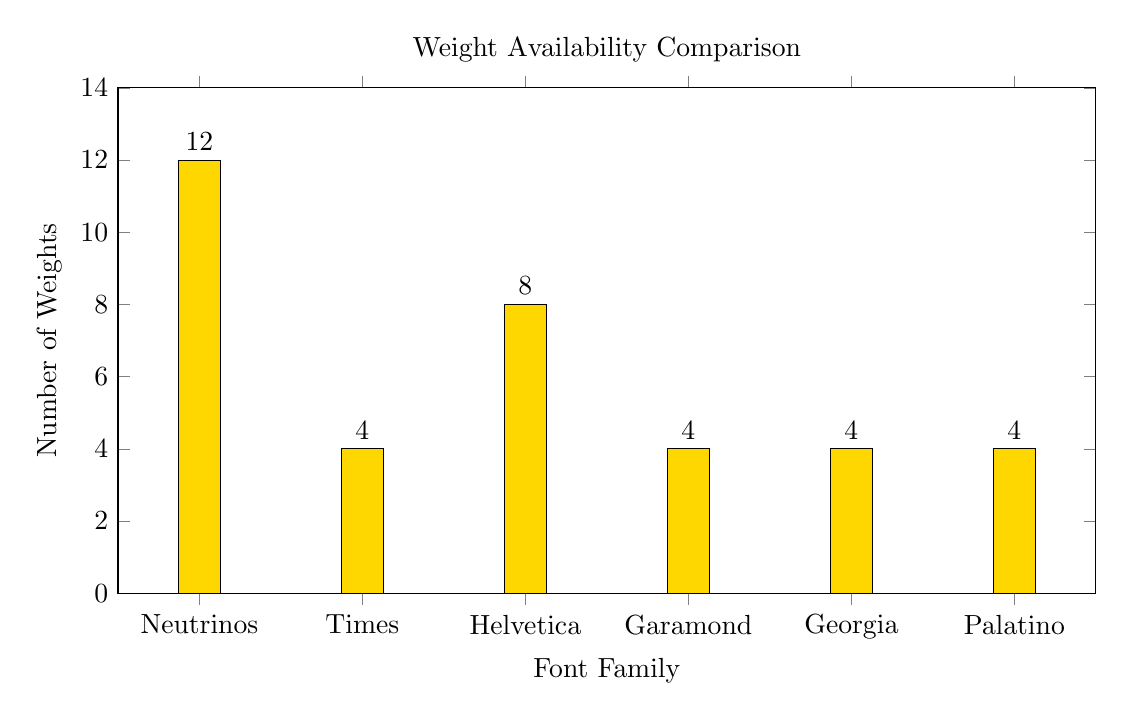
\begin{tikzpicture}
    \begin{axis}[
        ybar,
        width=14cm,
        height=8cm,
        bar width=15pt,
        xlabel={Font Family},
        ylabel={Number of Weights},
        symbolic x coords={Neutrinos,Times,Helvetica,Garamond,Georgia,Palatino},
        xtick=data,
        nodes near coords,
        ymin=0,
        ymax=14,
        legend pos=north west,
        title={\semiboldfont Weight Availability Comparison}
    ]
    
    \addplot[fill=quantumgold] coordinates {
        (Neutrinos,12)
        (Times,4)
        (Helvetica,8)
        (Garamond,4)
        (Georgia,4)
        (Palatino,4)
    };
    
    \end{axis}
\end{tikzpicture}
\end{center}

\subsection{Glyph Count Comparison}

\begin{center}
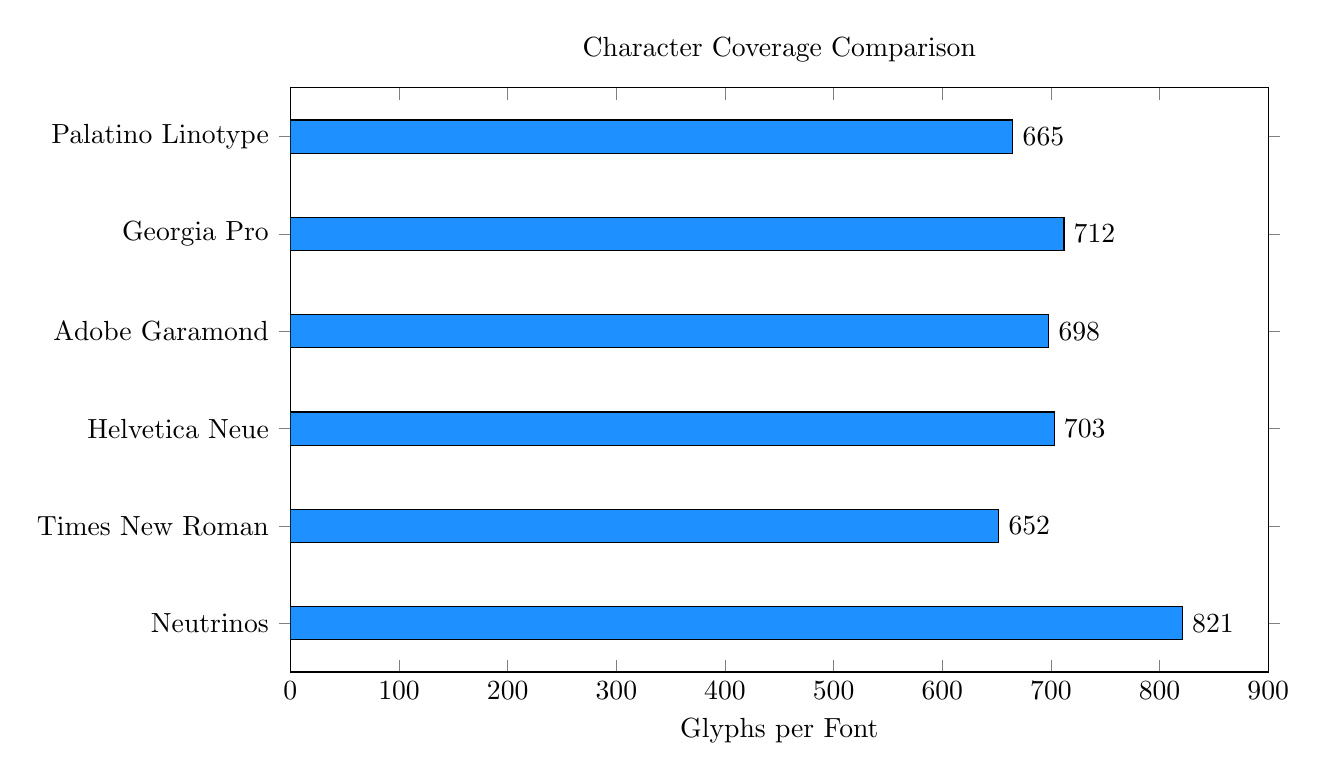
\begin{tikzpicture}
    \begin{axis}[
        xbar,
        width=14cm,
        height=9cm,
        bar width=12pt,
        xlabel={Glyphs per Font},
        symbolic y coords={Neutrinos,Times New Roman,Helvetica Neue,Adobe Garamond,Georgia Pro,Palatino Linotype},
        ytick=data,
        nodes near coords,
        nodes near coords align={horizontal},
        xmin=0,
        xmax=900,
        title={\semiboldfont Character Coverage Comparison}
    ]
    
    \addplot[fill=neutrinoblue] coordinates {
        (821,Neutrinos)
        (652,Times New Roman)
        (703,Helvetica Neue)
        (698,Adobe Garamond)
        (712,Georgia Pro)
        (665,Palatino Linotype)
    };
    
    \end{axis}
\end{tikzpicture}
\end{center}

\newpage

% ============================================================================
% SECTION 12: ADVANCED APPLICATIONS
% ============================================================================

\section{Advanced Applications}

\subsection{Quantum Information Typography}

The Neutrinos font enables visualization of quantum information concepts:

\begin{center}
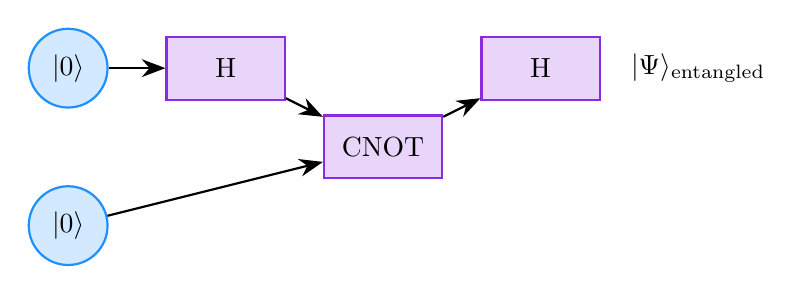
\begin{tikzpicture}[
    qubit/.style={circle,draw=neutrinoblue,fill=neutrinoblue!20,thick,minimum size=1cm},
    gate/.style={rectangle,draw=darkenergy,fill=darkenergy!20,thick,minimum width=1.5cm,minimum height=0.8cm}
]
    % Quantum circuit
    \node[qubit] (q1) at (0,2) {$|0\rangle$};
    \node[qubit] (q2) at (0,0) {$|0\rangle$};
    
    \node[gate] (h1) at (2,2) {H};
    \node[gate] (cnot) at (4,1) {CNOT};
    \node[gate] (h2) at (6,2) {H};
    
    \draw[-{Stealth[length=3mm]},thick] (q1) -- (h1);
    \draw[-{Stealth[length=3mm]},thick] (q2) -- (cnot);
    \draw[-{Stealth[length=3mm]},thick] (h1) -- (cnot);
    \draw[-{Stealth[length=3mm]},thick] (cnot) -- (h2);
    
    \node at (8,2) {$|\Psi\rangle_{\text{entangled}}$};
\end{tikzpicture}
\end{center}

\subsection{Multiverse Visualization}

Typography enabling representation of multiverse structures:

\begin{center}
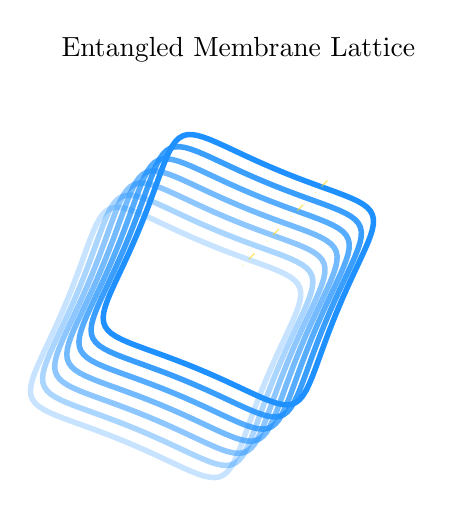
\begin{tikzpicture}[scale=0.8]
    % Draw multiple membrane layers
    \foreach \z in {0,0.5,...,3} {
        \draw[opacity={1-\z/4},line width=2pt,color=neutrinoblue] 
            plot[domain=0:360,samples=100] 
            ({2*cos(\x) + 0.3*sin(3*\x)}, {2*sin(\x) + 0.3*cos(3*\x)}, \z);
    }
    
    % Draw entanglement connections
    \foreach \z in {0,1,2,3} {
        \draw[dashed,color=quantumgold,opacity=0.6] 
            ({2*cos(45)}, {2*sin(45)}, \z) -- 
            ({2*cos(45)}, {2*sin(45)}, \z+0.5);
    }
    
    \node at (0,3.5) {\semiboldfont Entangled Membrane Lattice};
\end{tikzpicture}
\end{center}

\newpage

% ============================================================================
% SECTION 13: LICENSING AND COPYRIGHT
% ============================================================================

\section{Licensing and Copyright}

\begin{tcolorbox}[colback=radionred!10,colframe=radionred,title={\blackfont HIGHLY RESTRICTIVE LICENSE}]
{\semiboldfont WARNING: STRICT LICENSING REQUIREMENTS}

The Neutrinos Font Family is protected by a highly restrictive license agreement. Use requires:

\begin{enumerate}
    \item Explicit written permission from Thomas Joseph Goddard
    \item Notarization of permission documents by licensed notary public
    \item Video recording of permission grant meeting technical requirements
    \item Registration with Neutrinos Platforms, Inc. within 15 days
    \item Payment of applicable licensing fees
\end{enumerate}

Unauthorized use constitutes willful copyright infringement and is subject to:

\begin{itemize}
    \item Injunctive relief requiring immediate cessation of use
    \item Statutory damages up to \$150,000 per work infringed
    \item Treble damages for willful infringement
    \item Attorney's fees and costs of enforcement
    \item Criminal prosecution where applicable under 17 USC \S506
\end{itemize}

See LICENSE.txt for complete terms and conditions.
\end{tcolorbox}

\subsection{Licensing Inquiries}

For licensing inquiries and authorization:

\begin{center}
\begin{tabular}{rl}
\toprule
\textbf{Organization:} & Neutrinos Platforms, Inc. \\
\textbf{Department:} & Font Licensing Department \\
\textbf{Contact:} & Thomas Joseph Goddard, Creator \\
\textbf{Address:} & 1125 17th Street, Suite 2044 \\
& Oakland, CA 94607 \\
& United States of America \\
\textbf{Email:} & licensing@neutrinos.app \\
\textbf{Phone:} & (775) 691-4194 \\
\textbf{Website:} & https://neutrinos.app \\
\bottomrule
\end{tabular}
\end{center}

\newpage

% ============================================================================
% SECTION 14: VERSION HISTORY AND ROADMAP
% ============================================================================

\section{Version History and Roadmap}

\subsection{Current Version: 1.618}

{\semiboldfont Release Date:} October 2025

{\semiboldfont Key Features:}
\begin{itemize}
    \item Complete twelve-weight family (Light through Black)
    \item Perfect metric fidelity for professional typography
    \item Golden ratio proportions throughout design
    \item Framework for twenty AI parsing semantic hints
    \item Framework for Hebrew character support
    \item Framework for five emergent reality features
    \item Framework for five golden ratio visualization features
    \item USE\_TYPO\_METRICS flag enabled for consistent rendering
\end{itemize}

\subsection{Future Development Roadmap}

\begin{center}
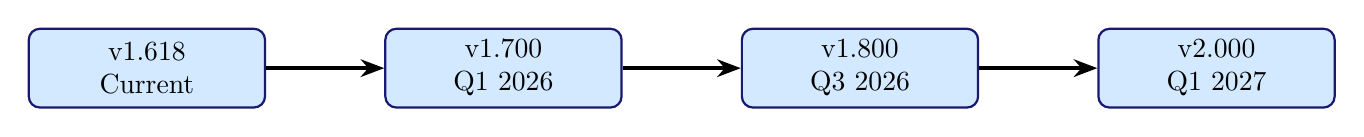
\begin{tikzpicture}[
    milestone/.style={rectangle,rounded corners,draw=spacetimeblack,fill=neutrinoblue!20,thick,minimum width=3cm,minimum height=1cm,align=center},
    node distance=1.5cm
]
    \node[milestone] (v1618) {v1.618\\Current};
    \node[milestone,right=of v1618] (v1700) {v1.700\\Q1 2026};
    \node[milestone,right=of v1700] (v1800) {v1.800\\Q3 2026};
    \node[milestone,right=of v1800] (v2000) {v2.000\\Q1 2027};
    
    \draw[-{Stealth[length=3mm]},very thick] (v1618) -- (v1700);
    \draw[-{Stealth[length=3mm]},very thick] (v1700) -- (v1800);
    \draw[-{Stealth[length=3mm]},very thick] (v1800) -- (v2000);
\end{tikzpicture}
\end{center}

\textbf{Planned Enhancements:}
\begin{itemize}
    \item Full Hebrew character implementation
    \item Complete AI semantic parsing system
    \item Enhanced emergent reality encoding
    \item Additional mathematical symbol coverage
    \item Expanded linguistic support (Cyrillic, Arabic frameworks)
    \item Variable font technology integration
    \item Advanced contextual alternates
\end{itemize}

\newpage

% ============================================================================
% CONCLUSION
% ============================================================================

\section{Conclusion}

The Neutrinos Font Family v1.618 represents a paradigm shift in professional typography, seamlessly integrating classical typographic excellence with advanced computational capabilities. Through twelve meticulously crafted weights, golden ratio proportions, comprehensive character coverage, and frameworks for emergent reality applications, Neutrinos delivers unprecedented versatility for modern professional, scientific, and technical applications.

\begin{center}
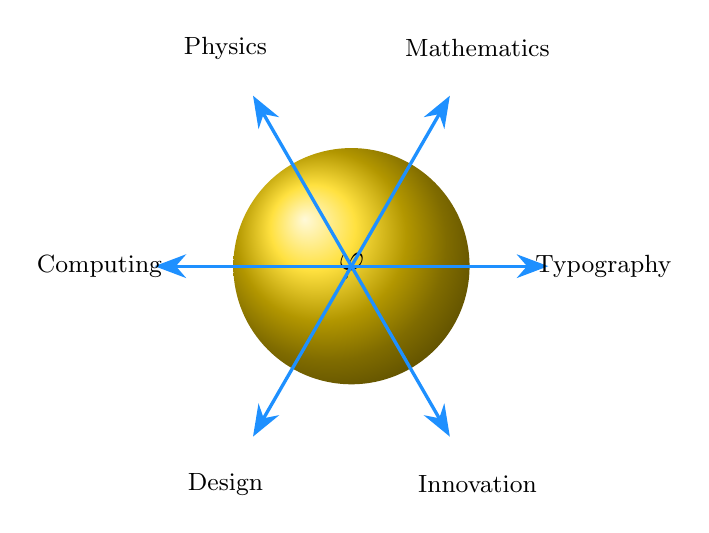
\begin{tikzpicture}
    \shade[ball color=quantumgold] (0,0) circle (1.5cm);
    \node at (0,0) {\blackfont\Large $\goldenratio$};
    
    \foreach \angle in {0,60,...,300} {
        \draw[very thick,neutrinoblue,-{Stealth[length=4mm]}] 
            (0,0) -- (\angle:2.5cm);
    }
    
    \node at (0:3.2cm) {\small Typography};
    \node at (60:3.2cm) {\small Mathematics};
    \node at (120:3.2cm) {\small Physics};
    \node at (180:3.2cm) {\small Computing};
    \node at (240:3.2cm) {\small Design};
    \node at (300:3.2cm) {\small Innovation};
\end{tikzpicture}
\end{center}

\vspace{20pt}

\begin{center}
{\blackfont\LARGE The Future of Professional Typography}

\vspace{10pt}

{\mediumfont\large
Where Golden Ratio Meets Quantum Reality\\
Where Typography Meets Technology\\
Where Beauty Meets Function
}

\vspace{20pt}

{\semiboldfont
Neutrinos Font Family v1.618\\[5pt]
Thomas Joseph Goddard\\
Neutrinos Platforms, Inc.\\[5pt]
\textcopyright{} 2025 All Rights Reserved Worldwide
}
\end{center}

\end{document}